\chapter{Integration of UML Profiles}\label{integration}
The following Chapter illustrates the concepts of the \ac{UML}
profiles integration into and with the aid of the tools introduced in the
previous chapter.
To achieve this, first an introduction is presented, which will show the basic 
ideas for the later sections in this chapter. Additionally an overview of
the integration process is given. This chapter concludes by presenting
the whole integration process in detail, which each tool has undergone.
\section{Introduction}\label{Integration:introduction}
Supporting as many modeling languages and therefore domains as possible is
crucial to all modeling tools, like the ones presented in chapter~\ref{environment_and_tools}.
The shift to \ac{MDSD} can only be accomplished, if modeling tools providing
needed features are supporting modeling languages of interest in practical use.
The \ac{UML} itself is very popular among developers because of its generic
approaches and its extensibility. As seen in
section~\ref{environment_and_tools:umlprofiles} has \ac{UML} taken the generic
approach of profiles as solution for integrating new domains and languages
into modeling tools, without the sacrifice of new tools needed.\\
Supporting \ac{UML} profiles is therefore an important step for each modeling
tool in practice. The following sections describe how this integration is done
in the previously presented modeling tools SiDiff, SiLift and the
Patch-Tool developed by the \ac{SEG}.
\section{Overview}\label{Integration:overview}
For a full \ac{UML} profiles integration through all tools used in the \ac{SEG},
each pipeline step has to be taken into consideration:
\begin{itemize}
  \item Profile support in \textbf{Matching} service
  \item Profile support in \textbf{Lifting} service
  \item Profile support in \textbf{Patching} service
\end{itemize}
An overview of the tool pipeline is presented in
the center of figure~\ref{integration_overview}.

\begin{figure}[h!]
\begin{center}
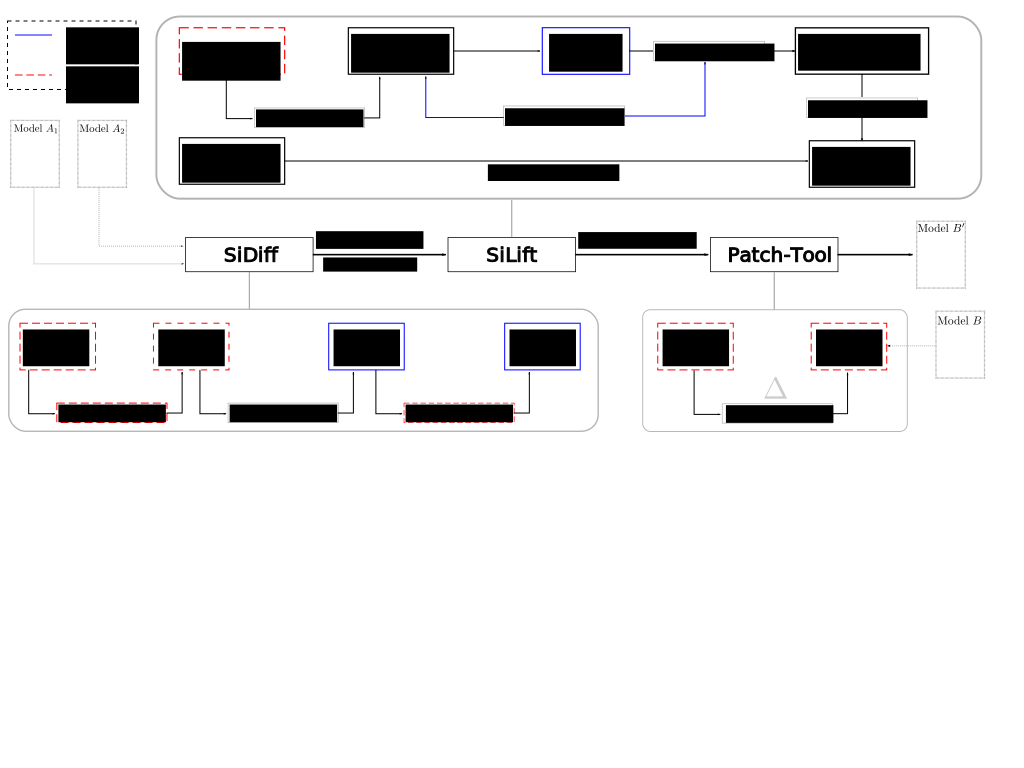
\includegraphics[scale=0.5, angle=0]{integration_overview}\\
\end{center}
\caption{UML profile integration overview}
\label{integration_overview}
\end{figure}
The tool pipeline can be described coarsely via the following steps:
\begin{enumerate}
  \item Two models $A_1$ and $A_2$ are given as input models.
  \item SiDiff creates a symmetric difference between them.
  \item SiLift lifts the low-level changes to more meaningful edit operations.
  \item The Patch-Tool deduces a patch and applies it to a target model $B$.
  \item The final result is a patched model $B'$ containing the changes
  detected between model $A_1$ and $A_2$ in model $B$ .
\end{enumerate}
As demonstrated in figure~\ref{integration_overview}, every tool has been
adapted for supporting \ac{UML} profiles, whether it be just modifications on
existing tools and services or creation of new ones. The concepts of this
adaptions will be presented in the following sections.
\section{SiDiff Integration}\label{Integration:sidiff}
The integration of \ac{UML} profiles into SiDiff and adaptions in general
can be divided into the following parts:

\textbf{\ac{UUID} Matcher}\\
The SiDiff matching pipeline has been adapted for better matching results if
elements of the input models contain \ac{UUID}s. Instead of just using one of
the matching services described in section~\ref{environment_and_tools:sidiff}, the
\ac{UUID} matching service is executed before the similarity-based matching
service. Therefore additional correspondences are already existent for the
following matching part, as shown in figure~\ref{integration_overview} in the
SiDiff box with dashed lines on the left side. Because of additional
correspondences at the start of of the similarity-matcher, it can deduce better
matching results. The already computed correspondences are taken into
consideration and are used as \textit{fix points} for the remaining unmatched
elements. This adaption is not specific for \ac{UML} profiles, but has been
implemented in this Master's Thesis.

\textbf{Similarity Matcher}\\
For the later concepts of the \ac{UML} profile integration and better matching
results in general, the similarity-based matcher has been adapted via its
configuration files. The focus was the definition of SiDiff configurations especially for
\ac{UML} itself, which can be used in other contexts as well. A snippet of such
a configuration is depicted in listing~\ref{sidiffcfg_example}.

\lstset{
    language=XML,    
    morekeywords={name,class,threshold,weight,parameter},
    caption={Snippet of \ac{UML} SiDiff configuration},
    label=sidiffcfg_example
    }
\lstinputlisting[firstline=633,lastline=640]{attachments/org.sidiff.sysml.core.compareconfig.xml}
In this example the matcher is configured for an \ac{UML} \textit{Class}
element, which will be matched after its attribute \textit{name}(l2-l3) and its
relationship to its \textit{parent} and \textit{children}(l4-l8). By adjusting
the weight between the configured elements, the results of the matching may improve or get worse.
This is just a small example of the vary configuration possibilities SiDiff has to offer. For a more detailed look into the possible SiDiff configuration parameters concerning the similarity
matching service contacting the \ac{SEG} via \cite{SEGURL} is suggested. As the
adaption of the \ac{UUID} Matcher, the improvement of the similarity-based matching
configuration for \ac{UML} is independent from the integration itself.

\textbf{Profile Matcher}\\
Profiled elements, conforming to the additive manner of \ac{UML} profiles, are
constructed as shown in figure~\ref{profilematcher_example1}: The base element
taken from \ac{UML}, in this case \textit{Class}, is extended by a newly defined
element, \textit{Block} in this case. Their relationship is defined via the
\textit{base\_Class} reference, which is a particular reference name used by
\ac{UML} profiles.

\begin{figure}[h!]
\begin{center}
\includegraphics[scale=1.0]{profilematcher_example1}\\
\end{center}
\caption{Example of two profiled models}
\label{profilematcher_example1}
\end{figure}

To describe the concept behind the developed profile matcher, two scenarios
concerning the example including model $A$ and model $B$ in figure~\ref{profilematcher_example1} can be imagined:
\begin{itemize}
  \item[a)] All elements contain \ac{UUID}s and they are corresponding to each other.
  \item[b)] One or all elements own a different \ac{UUID} or none at all.
\end{itemize}
In case a), which is presented in figure~\ref{profilematcher_example1}, the
newly integrated \ac{UUID} matcher will match corresponding elements. The
following execution of the similarity-based matcher will not add any new
results as already all possible correspondences have been found in the earlier
matching phase. Considering case b), in the similarity-based matching phase
there are unmatched elements because of wrong or missing \ac{UUID}s. Newly
introduced elements like \textit{Block} might be unmatched, in which case SiDiff
needs a feature to match those elements. To match profiling elements, there are
two possible solutions at hand:
\begin{enumerate}
  \item \textbf{Making use of the similarity matcher}\\  
  		Whereas at first sight this options seems more appropriate, the usage of the
  		similarity-based matching service depends highly on its configuration. As
  		explained beforehand, this configuration defines weighted elements and
  		attributes which should be taken into consideration for matching results. If
  		one element does not have much of its own semantics which can be considered
  		as important properties, the similarity matcher can not deduce meaningful
  		matches, which leads to wrong or missing correspondences between two models.
  		Taking figure~\ref{profilematcher_example1} into consideration, a element of
  		the type \textit{Block} does only define one boolean as own additional
  		attribute.
  		Comparing this attribute of model $A$, describing the additional semantics
  		of such \textit{Block}, to model $B$ one can clearly see that
  		this may lead to wrong correspondences. The only striking property of a \textit{Block} is the
  		reference to its base element. As such reference is always existent in
  		\ac{UML} profiling elements, the needed configuration of the similarity
  		matcher seems a unnecessarity. For each \ac{UML} profile and its elements
  		such a configuration part needs to be created, whereas they would contain
  		the same semantic content presented in listing~\ref{profiled_sidiffcfg}.
  		\lstset{
    language=XML,    
    morekeywords={name,class,threshold,weight,parameter},
    caption={SiDiff configuration for profiling elements},
    label=profiled_sidiffcfg
    }
    \begin{lstlisting}
    <Class name="Block" threshold="1.0">		
		<CompareFunction class="Parent" parameter="ECMatchedOrSimilar" weight="1.0"/>
		</Class>\end{lstlisting}
  \item \textbf{Implementing a new matching service}\\
  		Instead of using an available matching service, an additional matcher can be
  		introduced for supporting \ac{UML} profiles. As presented in
  		figure~\ref{integration_overview} an additional matcher for \ac{UML}
  		profiles has been developed and will be executed after the other matching
  		services provided by SiDiff. The basic idea behind the profile matcher is to
  		use all correspondences already created by other matchers and deduce results
  		concerning profiling elements from the former.
\begin{figure}[h!]
\begin{center}
\includegraphics[scale=1.0]{profilematcher_example5}\\
\end{center}
\caption{Concept of implemented profile matcher}
\label{profilematcher_example5}
\end{figure}

		The concept of the introduced profile matcher is shown in
		figure~\ref{profilematcher_example5}: The red marked boxes and correspondences
		have been created through the matchers prior in the SiDiff pipeline like the
		\ac{UUID} matcher or similarity matcher. If two elements are corresponding, which serve as base
		elements for profiling elements like in this case, the profiling elements
		marked in blue are also considered as corresponding. In this case the
		\ac{UML} configuration for SiDiff is crucial for good matching result, as
		the semantics of the base elements is used through the similarity matcher for
		matching the profiling elements. The profile matcher itself needs only a very minimal configuration
		effort, instead of the first variant using the similarity-based matching
		service. A detailed explanation of how this service is implemented and
		configurated can be found in section~\ref{realization:profilematcher}.
\end{enumerate}
\textbf{\ac{UUID} Fixer}\\
As the first two adaptions described in this chapter, this additional service
can be separated from the integration of \ac{UML} profiles. The \ac{UUID} fixer
service, as the name suggests, has been created for fixing wrong \ac{UUID}s
between corresponding elements. An explanatory example for a use case of the new
implemented service is presented in figure~\ref{wrongUUIDs_examples_p3}: Two
corresponding \textit{Associations}, namely Association2 and Association3, own
different identifiers. This can happen if an element has been deleted by the
developer and afterwards created newly again, representing the same semantics.
Many modeling tools rely on \ac{UUID}s and their correctness, whereas the
similarity matcher of SiDiff does not and creates such a correspondence
correctly. The new \ac{UUID} fixing service now corrects all \ac{UUID}s which
are mismatching, in this case it would replace the identifier of
Association3 with the one of Association2. Whether to change the \ac{UUID}s the
other way round is arguable, but the premise is to have two
consecutive revisions of software. In such a particular case, the identifiers in
the newer revision should be fixed instead of the ones in the older revision,
which would ruin all comparison possibilities with even older revisions.

\begin{figure}[h!]
\begin{center}
\includegraphics[scale=0.4]{wrongUUIDs_examples_p3}\\
\end{center}
\caption{Wrong \ac{UUID} example}
\label{wrongUUIDs_examples_p3}
\end{figure}

The service itself can be executed at any time considering the matching
pipeline, whereas its results are the best possible if executed at last.
By using this new service SiDiff itself offers a new feature, which has been
absent beforehand: Instead of supporting only matching of elements, SiDiff now
can fix wrong models and therefore make them yet again compatible to other
tools, which depend heavily on correct \ac{UUID}s.

For using all adapted and newly created tools together described in this section,
one can image following steps referring to the example in
figure~\ref{profilematcher_example1}, whereas the identifiers of the
\textit{Block} elements should differ:
\begin{enumerate}
  \item Both classes are matched by the \ac{UUID} matching service as they own
  the same identifier.
  \item The similarity-based matching service will not find any additional
  correspondences, because blocks are not part of the \ac{UML} configuration for
  SiDiff.
  \item Using the profile matcher, both blocks are matched because their
  respective base element \textit{Class} has been matched beforehand.
  \item Finally, the \ac{UUID} fixing service is executed and will replace the
  identifier of the \textit{Block} in model $B$ with the one of model $A$.
\end{enumerate}
Afterwards a generic \ac{UUID} matcher is capable of matching all elements,
including profiling ones like \textit{Block} in this example.
\section{SiLift Integration}\label{Integration:silift}
The integration of \ac{UML} profiles into SiLift translates to an integration
of \ac{UML} profiles into Henshin edit rules. If these rules are providing
support for profiled elements, then SiLift provides this support as well.
As already seen in figure~\ref{profilematcher_example1}, do profiled elements
essentially consist of themselves besides the relationship to their respective
base element. These two components need to be integrated into Henshin edit
rules, which can then be used by SiLift for its purposes. To achieve this goal,
three different variants can be deduced which are presented in
figure~\ref{variants_overview} using \ac{SysML} as applied \ac{UML} profile.

\begin{figure}[h!]
\begin{center}
\includegraphics[scale=1.0]{variants_overview}\\
\end{center}
\caption{Overview of different integration variants}
\label{variants_overview}
\end{figure}

\begin{enumerate}
  \item[Variant 1] \textbf{Integration into \ac{SERGe}}\\
 \ac{SERGe} is already capable of generating atomic edit rules by analyzing the
 corresponding meta model, including all \textit{set}, \textit{create}
 and \textit{delete} edit operations possibly executable by developers. Although
 \ac{UML} itself is supported by \ac{SERGe}, the profiling mechanism is not. The
 generator has to be adapted, to generate atomic edit rules, which contain the
 base elements as well as the profiling elements. The crucial advantage of this
 variant is the automated process of generating edit rules, whereas on the other
 hand new manually created edit rules can not be covered by this variant.
 Because of this drawback this variant has not been implemented in this Master's
 Thesis.
  \item[Variant 2] \textbf{Merging of Henshin rules}\\
  Another feasible solution is the merging of Henshin rules. The concept behind
  this idea is to take two rules, one containing only the base element and its
  properties, the other containing only the profiling element, and merge them
  into one resulting rule. Whether both rules have been generated or manually
  created does not concern, the drawback of the first variant is therefore absent.
  One difficulty to overcome in this variant is the merging of the rules
  itself: Finding the corresponding intersections between two rules as
  well as mapping parameters between them is complex in detail. Implementing
  this variant generically which does not only support the merging of Henshin
  rules for \ac{UML} profiles but rather supports the merging functionality for
  such Henshin rules in general makes this variant substantial sophisticated.
  Another mentionable disadvantage is the manual intervention for merging rules:
  The tool user has to be an expert on the used modeling domain, as he must
  define which rules should be merged into each other. These disadvantage have
  led to the following variant as solution, whereas this 
  variant could be taken into consideration for future work as presented in
  chapter~\ref{conclusionfuturework}.
  \item[Variant 3] \textbf{Adding profiling elements to existing Henshin rules}\\
  This variant has been implemented as part of this Master's Thesis as a service
  called \textit{ProfileApplicator}. Instead of merging two edit rules into one 
  as presented in variant 2, one pure edit base edit rule is taken as input and 
  transformed into a profiled one, containing profiling elements. This variant
  offers the same advantage like variant 2, the possibility of profiling
  manually created edit rules that is. Another advantage is the reduced complexity of
  development compared to the previous variant. Contrary to the merging variant,
  in this variant no manual intervention is needed in the creation process of
  the profiled rules, only a minimal configuration is needed for the
  ProfileApplicator to work instead. The concept of this variant is described in
  detail in the following section.
\end{enumerate}
\textbf{ProfileApplicator}\\
Adding profiling elements to a given model, which can be a Henshin rule itself,
can be achieved via a transformation. As Henshin is used in SiLift extensively
it has been chosen as the tool of choice for transformating such models. A Henshin
rule itself is a model, and therefore can be transformed like any other input
model. Such transformation is called \ac{HOT}, as it uses Henshin rules to
transform Henshin rules. An introductory result example of the execution of such
an \ac{HOT} is depicted in figure~\ref{hot_example}: The given edit rule on top
contains only the base element \textit{Class}, whereas the execution of a
\ac{HOT} adds the profiled element \textit{Block} to it resulting in the edit
rule shown below. 

\begin{figure}[h!]
\begin{center}
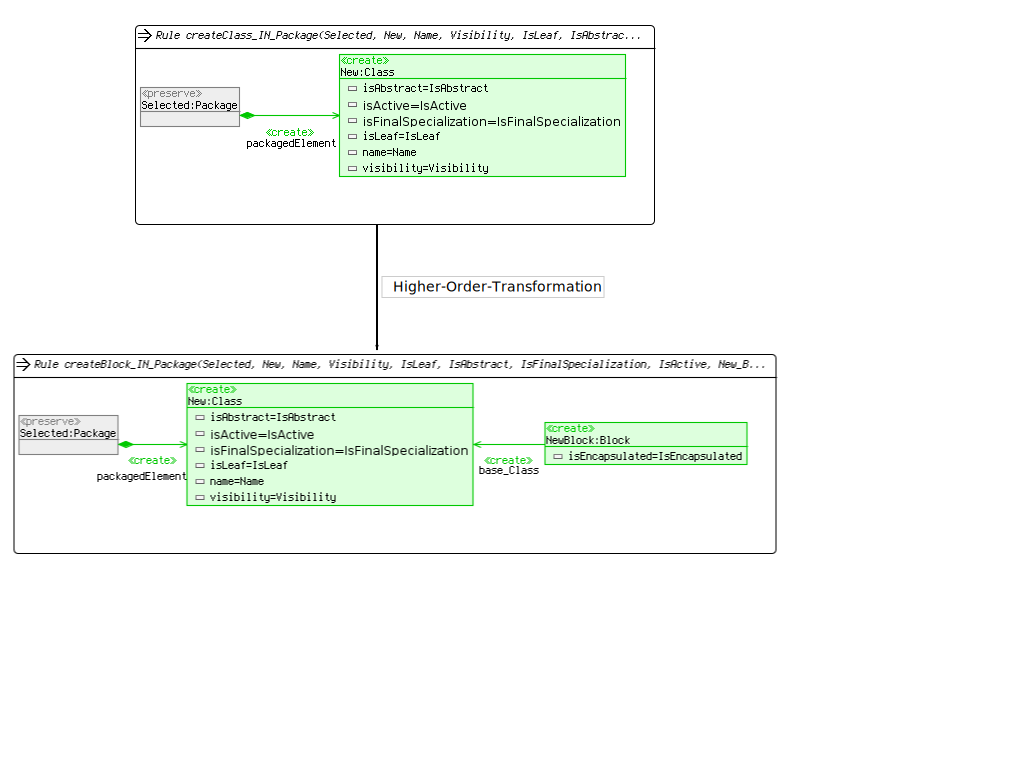
\includegraphics[scale=0.5]{hot_example}\\
\end{center}
\caption{\ac{HOT} example result}
\label{hot_example}
\end{figure}

This concept is implemented in the tool \textit{ProfileApplicator},
which executes such \ac{HOT}s for transforming given edit rules, such as
\ac{UML} edit rules.
As explained in section~\ref{environment_and_tools:henshin}, do Henshin rules
consist of three types of nodes: Create, delete and preserve. For each node type
a \ac{HOT} has been implemented, they can be found in
appendix~\ref{appendix:hots}. One exemplary rule covering the create nodes
depicted in figure~\ref{hot_create} will be explained in the following
paragraph.

Assuming the input model is an instance of a Henshin rule, the \ac{HOT} matches
a Module, which consists of one \textit{Unit} and one \textit{Rule}. Parts
of name and description attributes are replaced by a given String, this is just
a convenient renaming to identify profiled result rules more easily.
Additionally will the \ac{HOT} match a create node contained in the
\ac{RHS} graph and equals to the defined \textit{base type}, which is deducted
from the meta model of the \ac{UML} profile. If successful the following
elements will be created by this \ac{HOT}:
\newpage
\begin{itemize}
  \item A Create node of type \textit{stereo type} which has been derived from
  the meta model.
  \item An edge between the newly created node and the matched node of type
  \textit{base type}.
  \item All attributes of the stereo type node, except the ones defined as
  \textit{unchangeable}, \textit{derived} or \textit{transient} using a nested
  rule.
  \item New parameters in both the Henshin rule and unit.
  \item A parameter mapping between these two parameters.
\end{itemize}
The forbid node and edges are required for multiple executions of this \ac{HOT},
as there shall only be one profiled element of the same type be added to the
base element at most. If this \ac{HOT} is applied to the edit rule shown in the top of
figure~\ref{hot_example}, the rule below will be the result.

The remaining two \ac{HOT}s are defined in an similar manner, whereas some
differences can occur. The transformation of preserve nodes has to take also
the \ac{LHS} graph into consideration for example. Which base types will be used
as parameter can be configured in detail as will be seen in
section~\ref{realization:profileapplicator}.

 \textbf{Manually created edit rules}\\
 Although \ac{SERGe} does generate atomic edit rules by analyzing the
 corresponding meta model, not all rules containing the semantics are resulting.
 One example can be given in the area of the \ac{UML} concerning its
 representation of associations. An association is represented by two
 properties, which are either owned by the classes or by the association itself.
 Corresponding to optional relationships the meta model does not restrict the
 multiplicities, which results in \textit{wrong} generated edit rules. To cope
 with such special cases, one has to manually create such edit rules for
 themselves. One of the resulting rules is depicted in
 figure~\ref{atomic_example}: This edit rule is corresponding to the
 creation of an association which is navigable in one end. Such an association
 is defined via its properties, whereas one is owned by the corresponding class
 and the other is owned by the association itself. As part of this Master's
 Thesis different atomic manual rules have been created, which represent the
 semantics of the \ac{UML} meta model.
 
\begin{figure}[h!]
\begin{center}
\includegraphics[scale=0.55]{CREATE_Association_Navigable_ONE}\\
\end{center}
\caption{Manual atomic edit rule example}
\label{atomic_example}
\end{figure}

 Additionally to atomic edit rules, a domain expert can create complex edit
 rules, which have been defined in section~\ref{environment_and_tools:silift}.
 Adding complex edit rules, containing atomic edit rules, results in a better
 lifting possibility, which aids the developer at understanding the model more
 easily, as less edit operations are presented. One of the created rules is
 depicted in figure~\ref{complex_example}. As a special feature, this complex
 edit rule is modeled in \ac{SysML} instead of being modeled in \ac{UML} and
 transformated using the \textit{ProfileApplicator}. The reason for this is the
 added attribute \textit{direction} of the profiling element \textit{FlowPort}.
 This allows to define the direction of a given port and is a brilliant example for adding new
 semantics to known elements. This complex edit rule covers the creation of an
 interacting \textit{Block}, which is connected via its flow ports. The semantic
 behind this kind of block is that it receives a type of element, processes it in any
 way and passes the block on to another element connected via the outgoing port.
 This type of block is often used in the \ac{SysML} domain, as it may contain
 mechanical elements corresponding to this semantics.
 
 \begin{figure}[h!]
\begin{center}
\includegraphics[scale=0.5]{CREATE_Block_Interacting_Via_FlowPorts}\\
\end{center}
\caption{Manual complex edit rule example}
\label{complex_example}
\end{figure}

After manually creating missing edit rules and transformating all \ac{UML}
atomic and complex edit rules into profiled ones the defined rule base for \ac{UML}
profiles is complete. Now every possible edit operation in a particular
\ac{UML} profile like \ac{SysML} can be lifted with SiLift.
\section{Patch-Tool Integration}\label{Integration:patchtool}
Now that the first two steps of the tool pipeline
(fig.~\ref{integration_overview}) has undergone the \ac{UML} profile
integration, the final step has to be taken into consideration, the adaption
of the Patch-Tool that is. The Patch-Tool is responsible for the following three
features, which have to be adapted:
\begin{enumerate}
  \item \textbf{Creation of a patch} \\
  		The creation of a patch depends on the completeness of the given rule base
  		consisting of edit rules as well as the dependency correctness between them.
  		The latter as well as the former has successfully been solved through the
  		manual creation of rules missing or describing wrong semantics.
    \item \textbf{Application of a patch} \\
    	The successful application of a patch can only be ensured, if all
    	operation parameters can be resolved and the order of operations is correct
    	concerning the dependencies among them. Whereas the latter has already been
    	solved through the last feature, the former can be ensured if the matching
    	is done via SiDiff, including the \ac{UML} configuration and
    	profile matcher. Using these services a matching between all corresponding
    	elements can be created and therefore the parameter bindings.
    \item \textbf{Correctness of the result} \\
    	The last feature is the validation of the correct application of the patch.
    	For this purpose the models $A_1$ and $A_2$ are used for the creation of
    	such patch. The patch is then applied to $A_1$ and the result $B'$ is
    	compared to $A_2$. If and only if $A_2 = B'$ the patch has been applied
    	correctly and the result model contains all changes included in the patch.
    	A graphical overview of this situation is presented in figure~\ref{patch_correctness}.
		\begin{figure}[h!]
		\begin{center}
		\includegraphics[scale=0.6]{patching_correctness}\\
		\end{center}
		\caption{Patch result correctness condition}
		\label{patch_correctness}
		\end{figure}
		
		Such correctness can be only be tested as final step by using model instances,
		like done in chapter~\ref{solution}.
\end{enumerate}
 
\ac{UML} profiles are now fully integrated in all pipeline
steps(fig.~\ref{integration_overview}) and can be used consecutively. 
This chapter shall describe the concepts only instead of presenting the results
using a real \ac{SysML} case study. The results are explained extensive in
\ref{solution}.


